\documentclass[11pt,a4paper]{article}
\usepackage{ucs}
\usepackage[T1]{fontenc}
\usepackage[utf8x]{inputenc}
\usepackage[german]{babel}
\usepackage{amsmath}
\usepackage{amsfonts}
\usepackage{amssymb}
\usepackage{graphicx}
\usepackage{shadethm}
\usepackage{caption}
\usepackage{tikz} 
\usepackage{ziffer}
\usepackage{units}
\usepackage{multirow}
\usepackage{subfigure}
\usepackage{hyperref}
\usepackage{cleveref}
\usepackage{braket}

\newcommand{\minipanf}{\begin{minipage}{\linewidth}}
\newcommand{\minipend}{\end{minipage}}
\newcommand{\abs}[1]{\ensuremath{\left\vert#1\right\vert}}

\begin{document}

\include{EBIS_title} 	% Titelseite

\tableofcontents
\newpage 

\section{Einführung und Grundlagen}
	%TODO@Christian: Aufgabenstellung + EBIS Aufbau und Funktionsweise
    
    \subsection{Aufgabenstellung}
    Eine Elektronenstrahlionenquelle (EBIS) ermöglicht die Herstellung und Entnahme hochgeladener Ionen. Damit ist es möglich, die zeitliche Entwicklung von Ladungszuständen zu beobachten, woraus sich Aussagen über die Ionisationseigenschaften des Elektronenstrahls treffen lassen. \\
    Das Ziel dieses Versuches besteht darin, die Abhängigkeit der Ionisation von Ionisationszeit und Druck in der Ionenquelle zu untersuchen. Dafür werden zunächst die Betriebsparameter der Anlage eingestellt und die Extraktion des Ionenstrahls optimiert.
    Es folgt die Aufnahme eine Übersichtsspektrums der Ionen Ar$^{8+}$ bis Ar$^{18+}$ bei einer gegebenen, festen Ionisationszeit und einem mittleren Arbeitsdruck.
    Mit dem gleichen mittleren Druck wird die Zeitentwicklung der Ionenisationszustände 8+ bis 17+ aufgenommen.
    Danach erfolgt die Messung der Übersichtsspektren bei höherem und niedrigeren Arbeitsdrücken.
    \subsection{Aufbau und Funktionsweise des EBIS-A}
    
	\subsection{Elektrisch geladene Teilchen in einem homogenen Mag\-net\-feld}
		Um später die verschiedenen elektrisch geladenen Argonionen voneinander trennen zu können, ist im Niederenergiestrahlkanal ein 90°-Dipol-Magnet verbaut, der ein homogones Magnetfeld erzeugt und die Ionen auf eine Kreisbahn zwingt. Im Folgenden soll die Dynamik dieser Bewegung erörtert werden.\\
		Betrachte dafür ein elektrisch geladenes Teilchen mit Ladung $Q = q\cdot e$ und Masse $m$. Es wurde vorher von einem elektrischen Feld mit einer Spannung $U_B$ auf die Geschwindigkeit $\vec{v}(t=0)=v\vec{e}_x$ beschleunigt und befinde sich anschließend in einem homogenen Magnetfeld $\vec{B} = B \vec{e}_z$. In diesem erfährt es die \textit{Lorentzkraft}:
		\begin{equation}\label{eq:lorentz}
			\vec{F}_L(t) = Q\cdot\vec{v}(t)\times\vec{B} = QB(-v_x(t) \vec{e}_x + v_y(t)\vec{e}_y) = m\cdot \dot{\vec{v}}(t) \perp \vec{v}(t).
		\end{equation}
		Die z-Komponente ändert sich dabei nicht, somit findet die Bewegung o.B.d.A. in der x-y-Ebene statt. Da die Kraft zusätzlich zu jedem Zeitpunkt $t$ senkrecht zu der Geschwindigkeit ist, entsteht eine Bewegung auf einer Kreisbahn, deren Radius $R$ durch das Kräftegleichgewicht zwischen Lorentzkraft (\ref{eq:lorentz}) und der Zentrifugalkraft(\ref{eq:zentrifugal}) bestimmt wird:
		\begin{align}
			&\vec{F}_Z = - \frac{m\cdot v^2}{R}\cdot \frac{\vec{F}_L}{|\vec{F}_L|} \overset{!}{=} - \vec{F}_L \label{eq:zentrifugal}\\
			&\Rightarrow R = \frac{mv}{QB} = \sqrt{\frac{2U_Bm}{QB^2}}\label{eq:radius}
		\end{align}
		Wobei (\ref{eq:radius}) aus der Ersetzung der Geschwindigkeit durch die Beschleunigungspannung $U_BQ = mv^2/2$ erfolgte. Im Experiment ist der Radius $R = \unit[461]{mm}$ des Dipolmagneten vorgegeben, somit können durch Variation der Magnetflussdichte $B$ Teilchen einer bestimmten spezifischen Ladung $Q/m$ ausgefiltert werden. Dies wird später außerdem dazu genutzt, um Fremdionen im Übersichtsspektrum bei niedrigen Drücken identifizieren zu können, wobei die Zuordnung durch die Verhältnisbildung Masse zu Ladung nicht unbedingt eindeutig ist.
	
	\subsection{Wechselwirkungsprozesse von Ionen} \label{sec:ww}
		Trifft der Elektronenstrahl der EBIS auf die im Potentialtopf gebundenen neutralen Atome, beginnt die sukzessive Ionisation dieser bis sich in der Quelle ein stationärer Zustand zwischen Ionisations- und Rekombinationsprozessen einstellt. Um diesen Vorgang besser zu verstehen, sollen im Folgenden Abschnitt kurz die wichtigsten physikalischen Effekte diskutiert werden.\\
		Der in der Ionenquelle dominante \textbf{Ionisationsvorgang}, ist die sogenannte \textbf{Elektronenstoßionisation}. Dabei wird ein Elektron des Atoms oder Ions aus der Atomhülle durch Zusammenstoß mit einem Elektron des Kathodenstrahls herausgelöst. Die kinetische Energie des Strahlelektrons muss dabei größer sein als die Ionisationsenergie des Atoms.
		\begin{equation}
			\text{X}^{q+} + e^{-} \rightarrow \text{X}^{(q+1)+} + 2e^{-}
		\end{equation}
		Der \textbf{Augerprozess} stellt einen mehrstufigen Ionisationsvorgang dar. Dabei wird ein Atom durch einen Elektronenstoß in einen metastabilen angeregten Zustand versetzt und kehrt unter Aussendung eines sogenannten Augerelektrons eines äußeren Orbitals in den Grundzustand zurück.
		\begin{equation}
					\text{X}^{q+} + e^{-} \rightarrow (\text{X}^{q+})^* + e^{-} \rightarrow \text{X}^{(q+1)+} + 2e^{-}
		\end{equation}
		Prozesse, die der Erhöhung der Ladungszustände von Ionen entgegenwirken, nennt man \textbf{Rekombinationsvorgänge}. Der in der Quelle dominante Prozess dieser Art ist die \textbf{strahlende Rekombination}. Dabei wird ein Elektron aus dem Elektronenstrahl in der Hülle eines Ions eingefangen. Die dabei freiwerdende Bindungsenergie und überschüssige kinetische Energie des Elektrons wird in Form eines Photons emittiert.
		\begin{equation}
			\text{X}^{q+} + e^{-} \rightarrow \text{X}^{(q-1)+} + \hbar\omega
		\end{equation}
		Neben den Wechselwirkungen der Elektronen des Kathodenstrahles mit den Atomen in der Falle kommt es auch zu Interaktionen der Ionen untereinander. Ein Prozess dieser Art ist der \textbf{Ladungsaustausch}, der besonders hoch ionisierte Teilchen bei Zusammenstößen in niedrigere Ladungszustände versetzt. Dabei findet für $q<p$ folgende Reaktion statt:
		\begin{equation}
			X^{q} + X^{p} \rightarrow X^{q+1} + X^{p-1}.
		\end{equation}
		Der Wirkungsquerschnitt für diesen Prozess ist proportional zur Energie der Ionen und nimmt somit für hohe Arbeitsdrücke zu. Will man besonders hohe Ionisationszustände erreichen, ist es somit notwendig, den Druck so gering wie möglich zu halten.\cite{PA}
					% Physikalischer Hintergrund
\section{Versuchsdurchführung und Auswertung}
	\subsection{Einstellen der Betriebsparameter}
		Um die folgenden Messungen unter möglichst günstigen Bedingungen durchführen zu können, wurden zunächst unter Anweisung des Betreuers die Betriebsparameter der Ionenfalle überprüfung und gegebenenfalls optimiert:
		\begin{itemize}
			\item linke Potentialwand $U_0 = \unit[11,857]{kV}$
			\item Potentialtopf ($\hat{=}$ Beschleunigungsspannung) $U_A = \unit[11,707]{kV}=U_B$
			\item rechte Potentialwand $U_{B1} = \unit[12,007]{kV}$
			\item Extraktionszeit $t_{ext} = \unit[20]{ms}$
		\end{itemize}
		Da die Abhängigkeit der Argonionisationen von Arbeitsdruck und Ionisationszeit innerhalb des Strahlrohrs untersucht werden soll, werden diese in den folgenden Abschnitten genauer spezifiziert. Abbildung \ref{fig:potentialkasten} skizziert nochmals die Potentialverhältnisse entlang der Strahlachse.
		\begin{figure}[htb]
			\centering
			\includegraphics[width=0.8\linewidth]{pic/potentialkasten}
			\caption{Elektrodenanordnung (oben) mit zugehörigem Potentialverlauf in der Ionenfalle.\cite{PA}}
			\label{fig:potentialkasten}
		\end{figure}
		
	\subsection{Aufnahme und Analyse eines Übersichtsspektrums}
		Um die einzelnen Ionisationszustände des Argons sauber voneinander trennen zu können, ist es notwendig zu wissen, wie man den Strom des 90°-Dipol-Magneten wählen muss. Im Experiment sollen die Ionen Ar$^{8+}$ bis Ar$^{18+}$ untersucht werden. Mit Hilfe von Formel (\ref{eq:radius}) wird das Magnetfeld abgeschätzt, um die gewünschten Ionen auszufiltern. Es ergibt sich ein Messintervall von $B = 50,4 \dots \unit[75,6]{mT}$, wobei die untere Grenze den höchsten Ionisationszustand Ar$^{18+}$ und die untere Grenze den niedrigsten Zustand Ar$^{8+}$ herausfiltert. Die Einstellung dieser Magnetflussdichten erfolgt über die Variation des Spulenstroms von $\unit[17,3]{A}$ bis $\unit[27,2]{A}$. 
		Bei der ersten Messung wurde die Ionisationszeit mit $t_{ion} = \unit[380]{ms}$ zu hoch gewählt, um damit niedrigere Ladungszustände als Ar$^{13+}$ zu erzeugen. Dieser Effekt wird im zweiten Versuchsteil näher erörtert. Abbildung \ref{fig:7e-9} zeigt das dabei entstandene Übersichtsspektrum, welches bei mittlerem Arbeitsdruck von $p = \unit[7\cdot 10^{-9}]{mbar}$ entstanden ist. Die Ladung $Q$ wurde dabei über 5 Zyklen integriert.		
		Um ein vollständiges Übersichtsspektrum zu erhalten, wurde die Messung am Ende des Versuchstages mit einer niedrigeren Ionisationszeit $t_{ion} = \unit[80]{ms}$ und einem nicht signifikant erhöhten Arbeitsdruck $p = \unit[2\cdot 10^{-8}]{mbar}$ wiederholt. Diese Wahl maximiert die Häufigkeit von mittleren Ionisationszuständen um Ar$^{12}$ und ermöglicht die Messung aller möglicher Peaks. Abbildung \ref{fig:2e-8} zeigt das zugehörige Übersichtsspektrum, bei dem ebenfalls über 5 Zyklen integriert wurde.\\
		\begin{figure}[h]
		    \centering
		    \begin{minipage}{0.9\linewidth}
		        \centering
		        \includegraphics[width=0.8\linewidth]{pic/7e-9_beschriftet}
		        \caption{Übersichtsspektrum bei $p = \unit[7\cdot 10^{-9}]{mbar}$ und $t_{ion} = \unit[380]{ms}$. Die Peaks niedriger Ladungszustände verschwinden aufgrund der zu hohen Ionisationszeit.}
		        \label{fig:7e-9}
		    \end{minipage}
		    \vfill
		    \begin{minipage}{0.9\linewidth}
		        \centering
		        \includegraphics[width=0.8\linewidth]{pic/2e-8_beschriftet}
		        \caption{Übersichtsspektrum bei mittlerem Arbeitsdruck $p = \unit[2\cdot10^{-8}]{mbar}$ und $t_{ion} = \unit[80]{ms}$. Alle gewünschten Peaks sind erkennbar, da nun mittlere Ladungszustände am häufigsten auftreten.}
		        \label{fig:2e-8}
		    \end{minipage}
		\end{figure}
		\ \\
		Durch Ermitteln der Peakpositionen erhält man die Magnetflussdichten, die im zweiten Versuchsteil genutzt werden sollen, um die Ladungszustände zu isolieren. Um zu prüfen, ob die in Abbildung \ref{fig:2e-8} eingezeichnete Zuordnung korrekt ist, wurde ein quadratischer Fit der reziproken relativen Ladung $e/Q$, welche nach (\ref{eq:Q}) proportional zu $B^2$ ist, vorgenommen.
		\begin{equation} \label{eq:Q}
		\frac{1}{q} = \frac{e}{Q} = \frac{r^2 e}{2 U_B m_{Ar}}\cdot B^2 \simeq \unit[21,92]{\frac{1}{T^2}} \cdot B^2
		\end{equation} 
		Wobei $m_{Ar} = \unit[39,9]{u}$ die Masse von Argon ist. Abbildung \ref{fig:quadr_fit} zeigt das Ergebnis dieses Fits mit dem Ansatz $1/q = A\cdot B^2$. Dabei wurde die Proportionalitätskonstante mit $A = (21,7 \pm 0,1)\unit{/T^2}$ bestimmt, was nach (\ref{eq:Q}) sehr gut zum theoretischen Wert passt.\\
		%Einen weiteren Beleg für die gute Übereinstimmung der aufgenommenen Messwerte mit den aus (\ref{eq:radius}) theoretisch berechneten Werten zeigt Tabelle \ref{tab:data_fit}, welche beide direkt miteinander vergleicht.\\
		\begin{figure}[htb]
			\centering
			\includegraphics[width=\linewidth]{pic/quadr_fit.pdf}
			\caption{Quadratischer Fit, um Zuordnung der Peaks aus Abbildung \ref{fig:2e-8} zu verifizieren.}
			\label{fig:quadr_fit}	
		\end{figure}
		%\begin{table}[htb]
		%	\centering
		%	\begin{tabular}{c|c|c|c}
		%		$q = \frac{Q}{e}$ & $B_{experimentell}$ [mT] & $B_{theoretisch}$ [mT] & $1/q = e/Q$\\
		%		\hline 
		%		17	&	51,83	&	51,77	&	0,059\\
		%		16	&	53,39	&	53,36	&	0,062\\
		%		15	&	55,15	&	55,11	&	0,067\\
		%		14	&	57,09	&	57,05	&	0,071\\
		%		13	&	59,23	&	59,20	&	0,077\\
		%		12	&	61,67	&	61,62	&	0,083\\
		%		11	&	64,42	&	64,36	&	0,091\\
		%		10	&	67,52	&	67,50	&	0,100\\
		%		9	&	71,14	&	71,15	&	0,111\\
		%		8	&	75,52	&	75,47	&	0,12
		%	\end{tabular}
		%	\caption{Ermittelte Magnetflussdichten, die die gewünschten Ionisationszustände auf eine Kreisbahn mit korrektem Radius lenken.}
		%	\label{tab:data_fit}
		%\end{table}
	\subsection{Einfluss des Drucks auf die Ionenzustände im Strahlkanal}
		Um den Einfluss des Arbeitsdrucks im Niederenergiestrahlkanal zu untersuchen, wurden zwei weitere Übersichtsspektren mit gleicher Ionisationszeit von $t_{ion} = \unit[380]{ms}$ und Messzeit von $t_{mess} = \unit[2000]{ms}$ (5 Zyklen), aber mit verschiedenen Drücken aufgenommen. Abbildung \ref{fig:all} zeigt dabei den direkten Vergleich vom Spektrum mit niedrigem Arbeitsdruck $p_1 = \unit[2\cdot 10^{-9}]{mbar}$ (rot) und hohem Arbeitsdruck $p_2 = \unit[5\cdot 10^{-8}]{mbar}$ (blau).\\
		\begin{figure}[htb]
			\centering
			\includegraphics[width=\linewidth]{pic/all_beschriftet.png}
			\caption{Übersichtsspektrum mit $t_ion = \unit[380]{ms}$ unter verschiedenen Drücken $p_1 = \unit[2\cdot 10^{-9}]{mbar}$ (rot) und $p_2 = \unit[5\cdot 10^{-8}]{mbar}$ (blau). In blau beschriftete Peaks kennzeichnen mögliche Fremdionen im Strahlkanal.}
			\label{fig:all}	
		\end{figure}
		\ \\
		Es fällt auf, dass bei \textbf{niedrigen Drücken} ein viel geringerer Ionenstrom durch die Anlage fließt und somit am Faradaycup weniger Ladung pro Zeiteinheit nachgewiesen wird. Die kinetische Gastheorie liefert einen Zugang, um dies zu verstehen: Druck ist ein Maß für die Kraft, die Gasmoleküle auf die Gefäßwand ausüben. Je niedriger der Druck, desto weniger Kollisionen der Teilchen gibt es mit der Gefäßwand und auch untereinander. Dies führt zu einer geringeren mittleren Geschwindigkeit der Gasteilchen und somit zu einer geringeren Stromdichte $j = n\cdot Q \cdot v$, welche am Faradaycup als Ladung pro Zeiteinheit und Fläche nachgewiesen wird. Doch warum tritt diese Absenkung hauptsächlich bei mittleren Ionenzuständen (Ar$^{13+}$ bis Ar$^{15+}$) auf? Dies kann über die Verringerung des \textit{Ladungsaustauschs} zwischen den Ionen, der in Abschnitt \ref{sec:ww} näher erläutert wird, begründet werden. Die Häufigkeit dieses Prozesses sinkt bei niedrigem Druck, wodurch hochgeladene Ionen begünstigt werden und die Absenkung des Ionenstroms kompensiert wird.\\
		In Abbildung \ref{fig:all} ist bei etwa $\unit[51]{mT}$ ein roter Peak deutlich zu sehen. Diesen könnte man naiverweise aufgrund des niedrigen Drucks dem höchst angeregten Argonzustand Ar$^{18+}$ zuordnen. Das ist allerdings nicht der Fall, da die Theorie diesen bei etwa $\unit[50,4]{mT}$ erwarten würde. Man kann spekulieren, ob der Peak zu einem höchst angeregten Fremdion aus dem Strahlkanal gehört. Ein Atom, bei dem diese Zuordnung hervorragend funktioniert, ist Sauerstoff mit einer Masse von $m_O = \unit[16]{u}$. Der Peak zu O$^{7+}$ ist genau an der erwarteten Position und auch sonstige Maxima des Sauerstoffs passen sehr gut in das gemessene Spektrum herein, fallen aber teilweise mit denen des Argons zusammen.\\
		Bei \textbf{hohem Druck} ist nicht nur die mittlere Geschwindigkeit, sondern auch die Teilchenzahl und somit auch die Zahl an Fremdatomen im Strahlkanal deutlich höher. Da der Ladungsaustausch nun begünstigt wird und zudem der Ionenstrom größer ist, treten Peaks von gering angeregten Fremdionen als starkes Untergrundrauschen vor allem im Bereich hoher Magnetfelder auf. Das führt dazu, dass mittlere und niedrige Argonionisationszustände, die durch die hohe Ionisationszeit ohnehin unterdrückt sind, nicht mehr sauber herausgeefiltert werden können. In Abbildung \ref{fig:all} wurde ein Versuch unternommen, mögliche Fremdionen mit Saustoff-, Stickstoff- und Kohlenstoffatomen zu identifizieren. Dies ist allerdings rein spekulativ, da die Peaks nur sehr klein sind und man zu noch höheren Magnetfeldern hätte übergehen müssen. Außerdem fallen viele Maxima aufgrund gleicher spezifischer Ladung $Q/m$ zusammen, wodurch keine eindeutige Zuordnung möglich ist.\\
		Da die Anzahl der Ionen proportional zur am Faradaycup gemessenen Ladung ist, erhält man durch Verhältnisbildung eine grobe Abschätzung der Anzahl an Fremdatomen. Dafür sucht man Peaks, die mit keinem anderen Fremdatom zusammenfallen und die nach Möglichkeit dem am häufigsten auftretenden Ionenzustand entsprechen, z.B. von O$^{7+}$ und Ar$^{16+}$.
		\begin{equation}
			\frac{N_{O}}{N_{Ar}} = \frac{Q(\text{O}^{7+})}{Q(\text{Ar}^{16+})}\approx \unit[15,4]{\%}
		\end{equation}
		Das heißt, es befindet sich tatsächlich noch ein signifikanter Anteil an Fremdatomen im Strahlkanal, der mit den untersuchten Ionen wechselwirkt.
		
	\subsection{Einfluss der Ionisationszeit auf die Ladungszustandsverteilung und Erzeugung}
        Um den Einfluss der Ionisationszeit $t_{Ionisation}$ auf auf die Erzeugung von Ladung zu untersuchen, hält man Druck und Ladungszustand jeweils konstant und variiert lediglich die Ionisationszeit. In den folgenden Diagrammen wurde auch die Schrittweite und die minimale sowie die maximale Ionisationszeit variiert, was in Tabelle \ref{zeit} ablesbar ist. Dies hat vor allem im direkten Vergleich der Abbildungen \ref{timed} Effekte auf die Güte und natürlich auf die Dauer der Messungen. Die zackige Struktur in Abbildung \ref{timeds} resultiert aus Messfehlern, die durch die Messelektronik verursacht werden, wenn diese zwischen verschiedenen Messbereichen hin- und herschaltet. Es kann auch an einer mangelhaften Übergabe der Einstellung der Ionisationszeit vom LabView-Prgramm an die Steuereinheit liegen. Diese Zackenstruktur ist demnach kein physikalisches Phänomen, sondern kann durch eine Optimierung - wie später für die Aufnahme der Zeitentwicklungen in Abbildung \ref{timedw} geschehen - vermieden werden.
        \begin{table}
                    \begin{tabular}{c|c|c|c|c|c|c}
                            \textbf{Q} & \label{B} [mT] & \textbf{t$_\text{start}$} [ms] & \textbf{t$_\text{stop}$} [ms] & \textbf{Stepsize} [ms] & \textbf{Zyklen} & \textbf{Falle auf} \\ 
                    \hline 8+ & 75,52 & 200 & 10 & 5 & 10 & 20 \\ 
                           9+ & 71,14 & 200 & 10 & 5 & 10 & 20 \\ 
                          10+ & 67,52 & 200 & 10 & 5 & 10 & 20 \\ 
                          11+ & 64,42 & 250 & 10 & 5 & 10 & 20 \\ 
                          12+ & 61,67 & 400 & 10 & 10 & 10 & 20 \\ 
                          13+ & 59,23 & 500 & 10 & 10 & 10 & 20 \\ 
                          14+ & 57,09 & 1000 & 20 & 20 & 7 & 20 \\ 
                          15+ & 55,15 & 1000 & 20 & 20 & 7 & 20 \\ 
                          16+ & 53,39 & 1500 & 25 & 25 & 5 & 20 \\ 
                          17+ & 51,81 & 2000 & 50 & 50 & 5 & 20
                \end{tabular} 
                \caption{Einstellungen zur Aufnahme der Kurven in Abbildung \ref{timed}}      
                \label{zeit}
        \end{table}
        Der Druck wurde konstant bei $p = 2\cdot10^{-8}\unit{mbar}$ gehalten.                   
        \begin{figure}
            \subfigure[Peaks der Zustände 8+ bis 11+\label{timeds}]{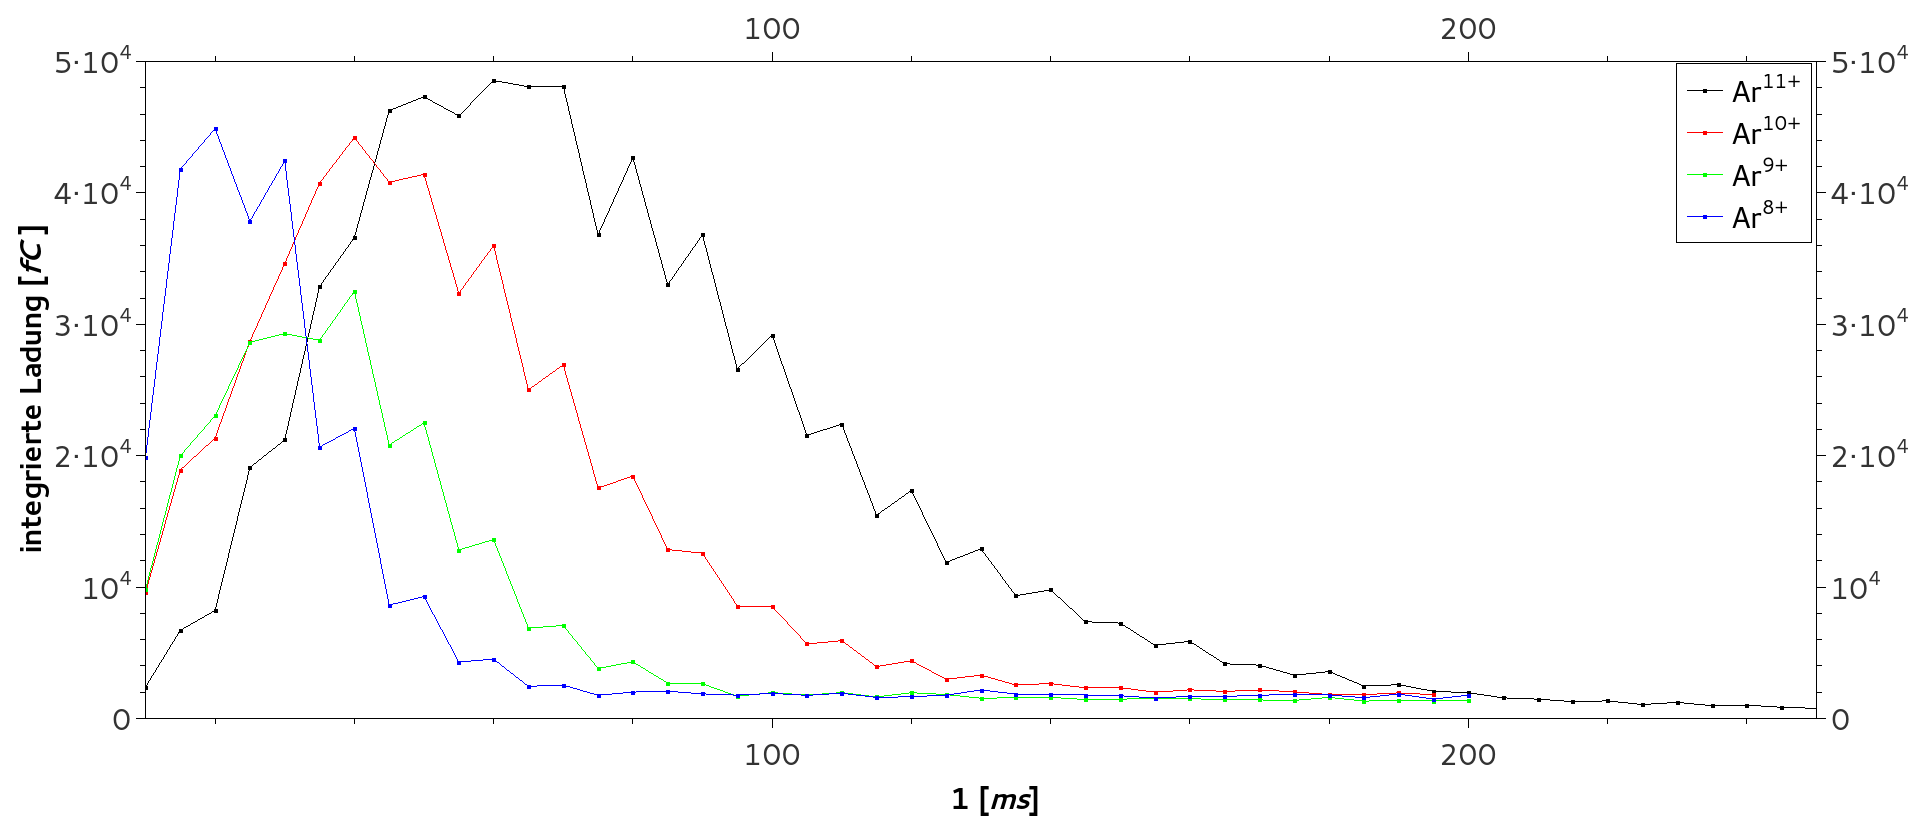
\includegraphics[scale=0.25]{pic/schmalePeaks.png}}
            \subfigure[Peaks der Zustände 12+ bis 17+\label{timedw}]{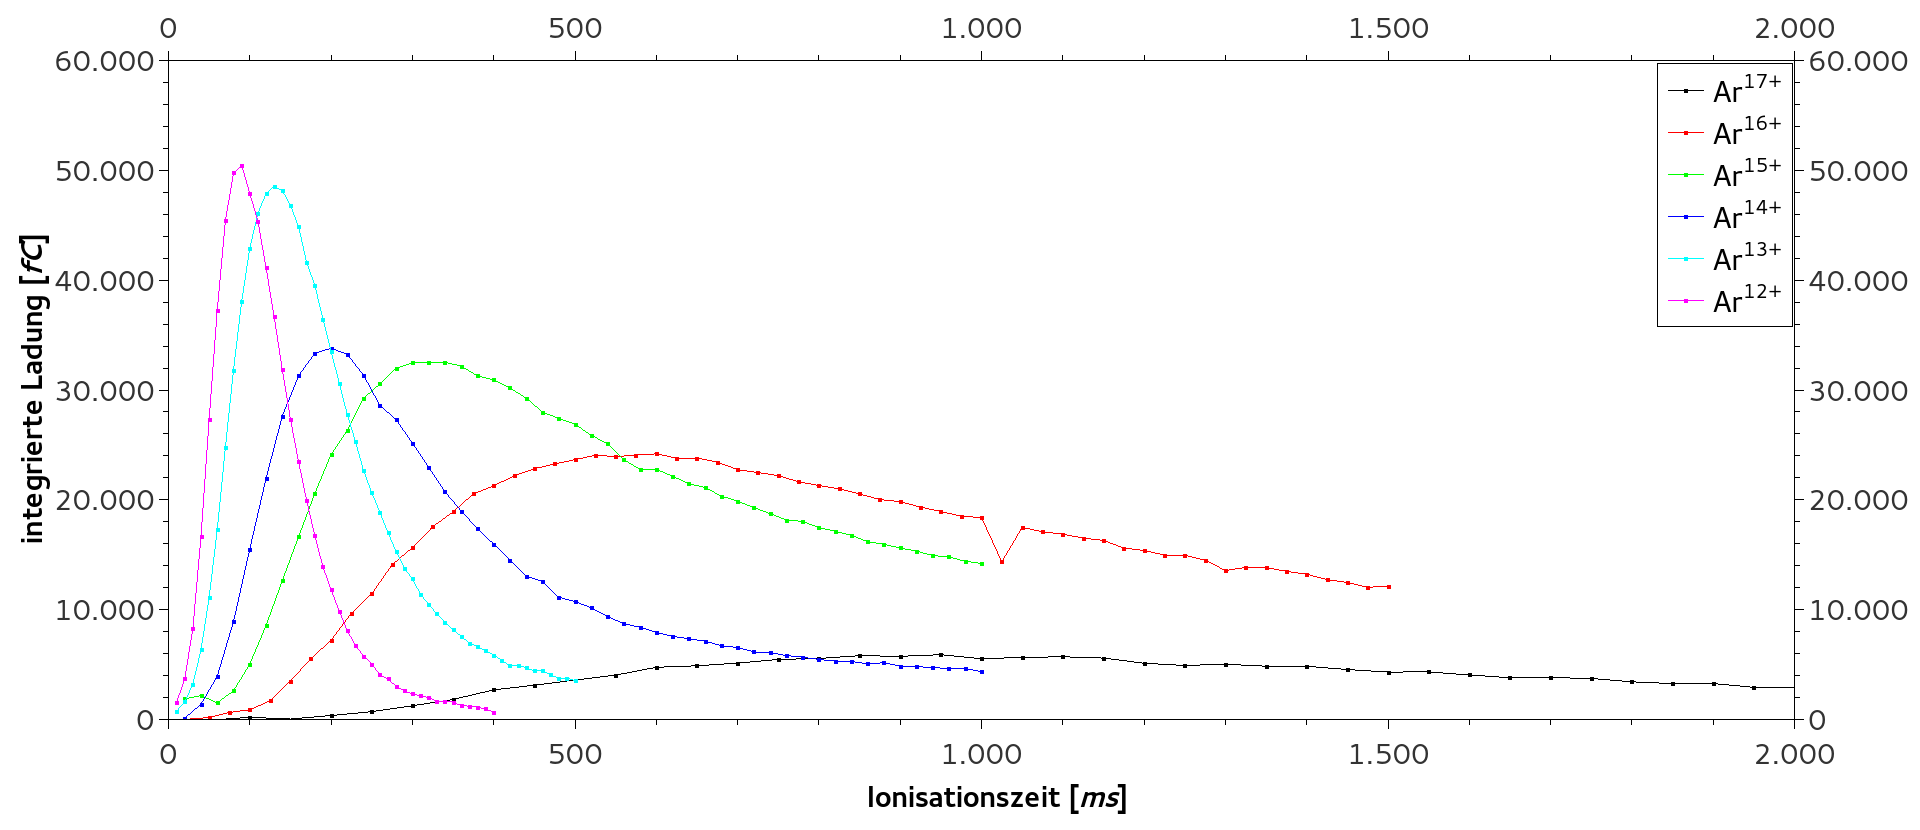
\includegraphics[scale=0.25]{pic/breitePeaks.png}}
            \caption{Einfluss der Ionisationszeit auf die Erzeugung von Ladung verschiedener Ladungszustände}
            \label{timed}
        \end{figure}
        Es ist qualitativ auffällig, dass jede Ionisationsstufe über einen mehr oder weniger ausgeprägten Peak verfügt. Die Messkurven verlaufen asymmetrisch und steigen links der Maxima wesentlich steiler an als sie rechts fallen. Besonders die niedrigen Ionisationsstufen Ar$^{8+}$ bis Ar$^{10+}$ und Ar$^{12+}$ zeigen rechts der Maxima gut erkennbar nahezu konstantes Verhalten in einiger Entfernung zum Peak. Das bedeutet, das sich mit steigender Ionisationszeit ein Gleichgewicht zwischen Rekombination und Ionisation einstellt.\\
        Qualitativ ist in Abbildung \ref{timed} auch erkennbar, dass die Maxima mit Zunahme der Ionisierung kleiner werden. Ebenso werden die Abstände zwischen den Peaks größer. Diese beiden Beobachtungen sind in Abbildung \ref{maxrel} zusammengetragen dargestellt.\\
        \begin{figure}
            \centering
            \subfigure[Zeitliche Entwicklung der Ladungszustandsverteilung\label{maxrel}]{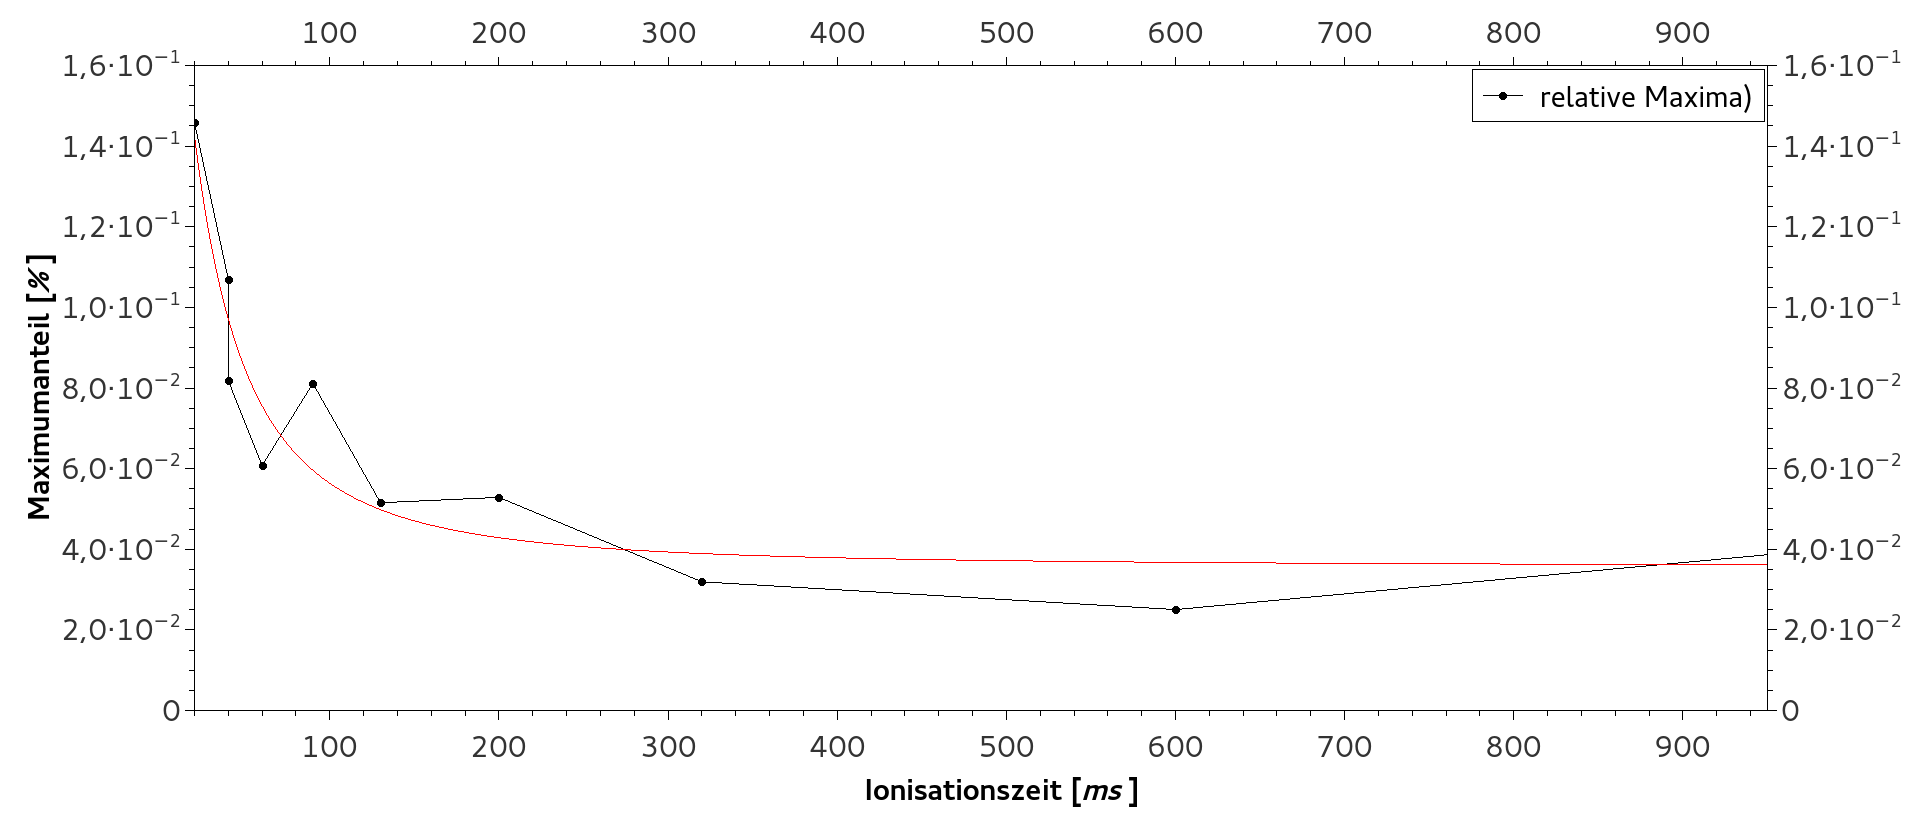
\includegraphics[scale=0.25]{pic/MaximaFit_relativ.png}}
            \subfigure[Maxima der Peaks in Abhängigkeit des Ladungszustandes\label{maxlad}]{\includegraphics[scale=0.452]{pic/LadungszustandsverteilungLinExp.png}}
            \caption{Maxima über Ionisationszeit und Ladungszustand}
            \label{max}
        \end{figure} 
        Hierbei ist anzumerken, dass die Ionisationsstufe mit der Ionisationszeit steigt, was man in Abbildung \ref{maxlad} erkennen kann. Aufgetragen wurden die Maxima der in Abbildung \ref{timed} dargestellten Graphen. Da die Messungen jedoch alle unter verschiedenen Bedingungen stattfanden, insbesondere da die Zyklenzahl verändert wurde, muss man die Höhe der Maxima normieren. In diesem Fall geschah dies relativ. Jedes Maximum ist geteilt durch die pro Ion für alle Ionisationszeiten gemessene Gesamtladung und aufgetragen worden. Daraus entsteht der hier erkennbare exponentielle Abfall mit einem Ausreißer.
        Dieses verhalten ist wiederum mit der steigenden Neigung der Ionen höherer Ordnung zur Rekombination erklärbar. Es dauert ebenfalls länger, höhere Ionisationsstufen herzustellen, wodurch die steigenden Ionisationszeiten für die Maxima erklärt werden können. 
        
        
        
        		% Durchführung
\input{EBIS_Protokoll_ausw}				% Auswertung
\section{Diskussion und Zusammenfassung}
	Im Experiment wurde die Abhängigkeit der Ionisationszustände Ar$^{8+}$ bis Ar$^{17+}$ in der EBIS von der Ionisationszeit und dem im Strahlkanal vorherrschenden Druck untersucht. Zu diesem Zweck wurden im ersten Versuchsteil Übersichtsspektren, die die am Faradaycup gemessene Ladung $Q(B)$ in Abhängigkeit vom Dipol-Magnetfeld $B$ darstellen, bei verschiedenen Drücken und konstanter Ionisationszeit aufgenommen. Dabei wurden zwei Effekte bei steigendem Druck beobachtet: Zum einen erhöht sich der Ionenstrom und somit die nachgewiesene Ladung, da die mittlere Geschwindigkeit der Teilchen zunimmt und zum anderen wird der Einfluss des Ladungsaustausches größer, wodurch höhere Ionisationszustände unterdrückt werden. Dies führte dazu, dass die Fremdatome (vor allem Sauerstoff) im Strahlkanal ein starkes Untergrundrauschen erzeugt haben. Will man somit besonders hohe Ionisationszustände erreichen, muss der Druck bzw. die mittlere Energie der Teilchen im Kanal herabgesetzt werden. Eine Möglichkeit dafür stellt die sogenannte \textbf{Ionenkühlung} dar, bei der leichte Fremdionen im Potentialtopf gebunden werden, welche die Energie der schweren Ionen aufnehmen und die Falle dabei verlassen. Dadurch wird dem System kontinuierlich Energie entzogen - die Ionen werden gekühlt - und sie verbleiben länger im Quellvolumen, sodass höhere Ladungszustände erreicht werden können. Diese Möglichkeit ist vor allem für sehr schwere Kerne wie Uran essentiell nutzbar. \cite{PA}\\
	Weiterhin wurde mit Hilfe der Übersichtsspektren die Theorie der Ablenkung geladener Teilchen im Magnetfeld des Dipol-Magneten sehr gut bestätigt, da die mit Formel (\ref{eq:radius}) berechneten Magnetfelder sehr gut mit dem quadratischen Fit aus Abbildung \ref{fig:quadr_fit} korrespondieren.\\
	Das Experiment, welches die Abhängigkeit der Erzeugung und Ladungszustandsverteilung untersucht hat, zeigt für die Erzeugung der Ionen deutlich an, dass sich bei einer gewissen Zeit ein Optimum (Maximum) herausbildet. Für Ionen niedrigerer Ordnung ist das Maximum ein deutlicher, nur leicht asymmetrischer Peak, während für die höheren Ordnungen die Amplituden exponentiell abfallen. Ebenso stellt sich heraus, dass zu lange Ionisationszeiten negativ auf die Erzeugung möglichst vieler Ionen wirken. Ist die Ionisationszeit zu lang, können sich Ionen höherer Ordnung bilden, oder andere Ionen können rekombinieren. In jedem Fall stellt sich dadurch ein Gleichgewicht zwischen Ionisation und Rekombination ein\\
    Die Ladungszustandverteilung (Abbildung \ref{maxrel}) zeigt einen exponentiellen Abfall, der ebenfalls mit der Ionisationszeit korrespondiert. 
	%TODO:Christians Diskussion		% Diskussion
\begin{thebibliography}{99}
\bibitem [01] {PA} Dr. Günter Zschornack. \textit{Elektronenstrahlquelle EBIS-A}. Großröhrsdorf, zuletzt geöffnet: 03.03.2016
\end{thebibliography}

\end{document}
